%!TEX root = ../../../report.tex

\begin{figure}[H]
	\captionsetup[subfigure]{aboveskip=-0.8em,belowskip=0.5em}
	\newcommand{\figurewidth}{0.5\textwidth}
	\begin{subfigure}[b]{\figurewidth}
		\figureborder{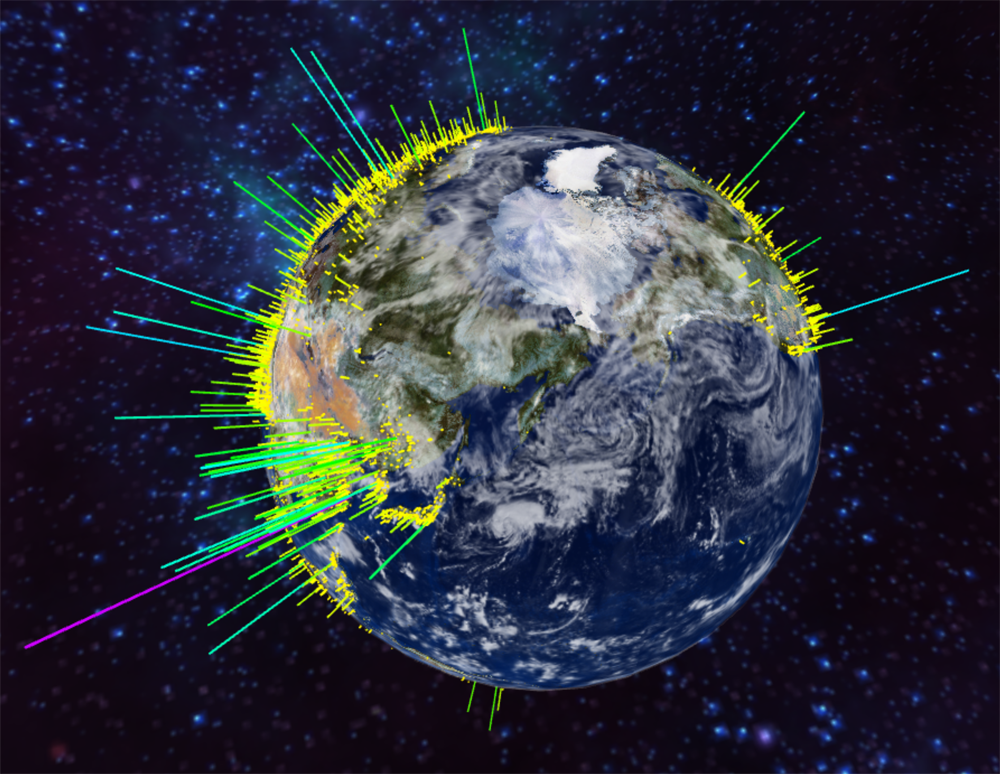
\includegraphics[width=\textwidth]{images/implementation/filtering/magnitude_before}}
		\caption{Before filtering the magnitude.}
		\label{fig:before_filtering_magnitude}
	\end{subfigure}
	\begin{subfigure}[b]{\figurewidth}
		\figureborder{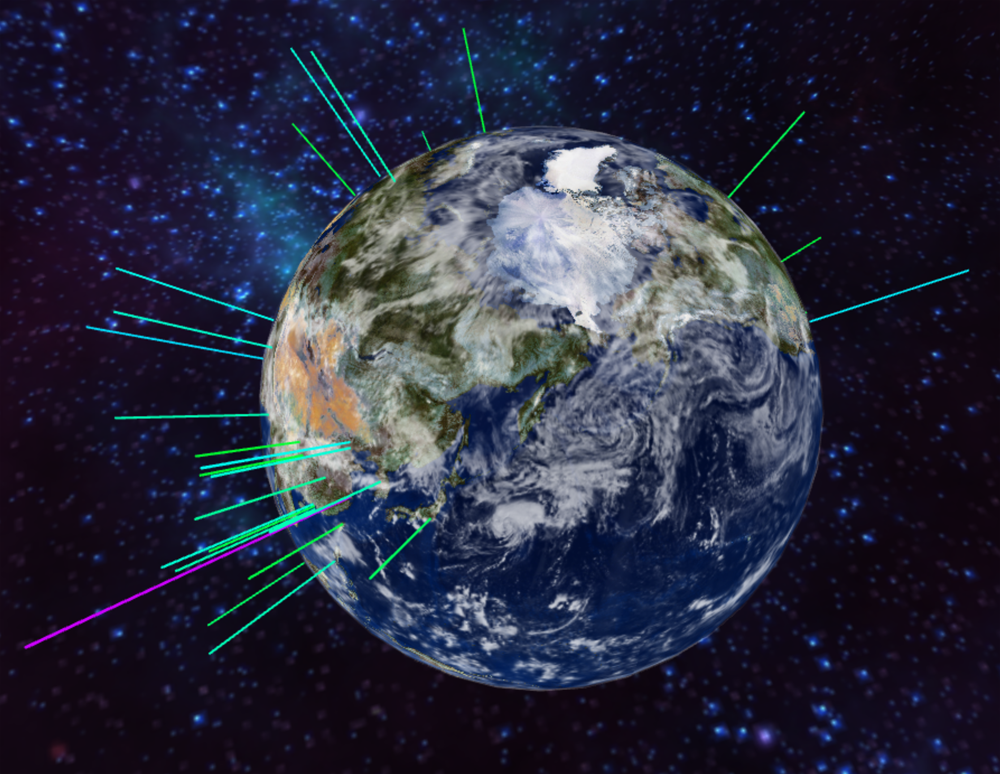
\includegraphics[width=\textwidth]{images/implementation/filtering/magnitude_after}}
		\caption{After filtering the magnitude}
		\label{fig:after_filtering_magnitude}
	\end{subfigure}
	\begin{subfigure}[b]{\figurewidth}
		\figureborder{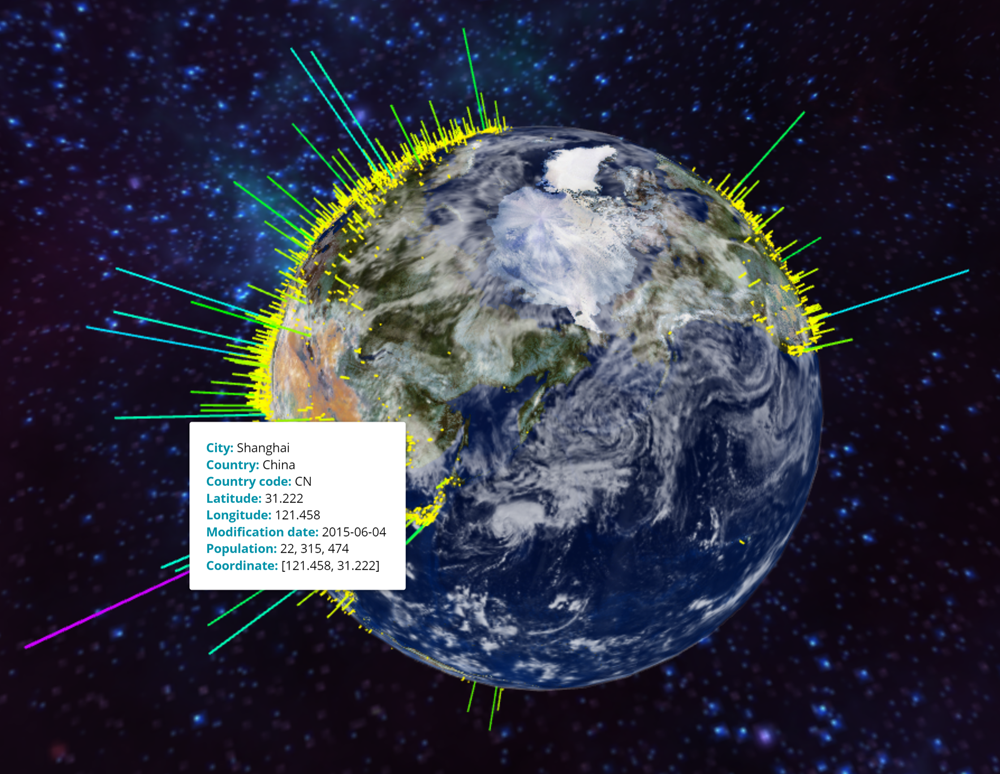
\includegraphics[width=\textwidth]{images/implementation/filtering/information_before}}
		\caption{Before filtering information.}
		\label{fig:before_filtering_information}
	\end{subfigure}
	\begin{subfigure}[b]{\figurewidth}
		\figureborder{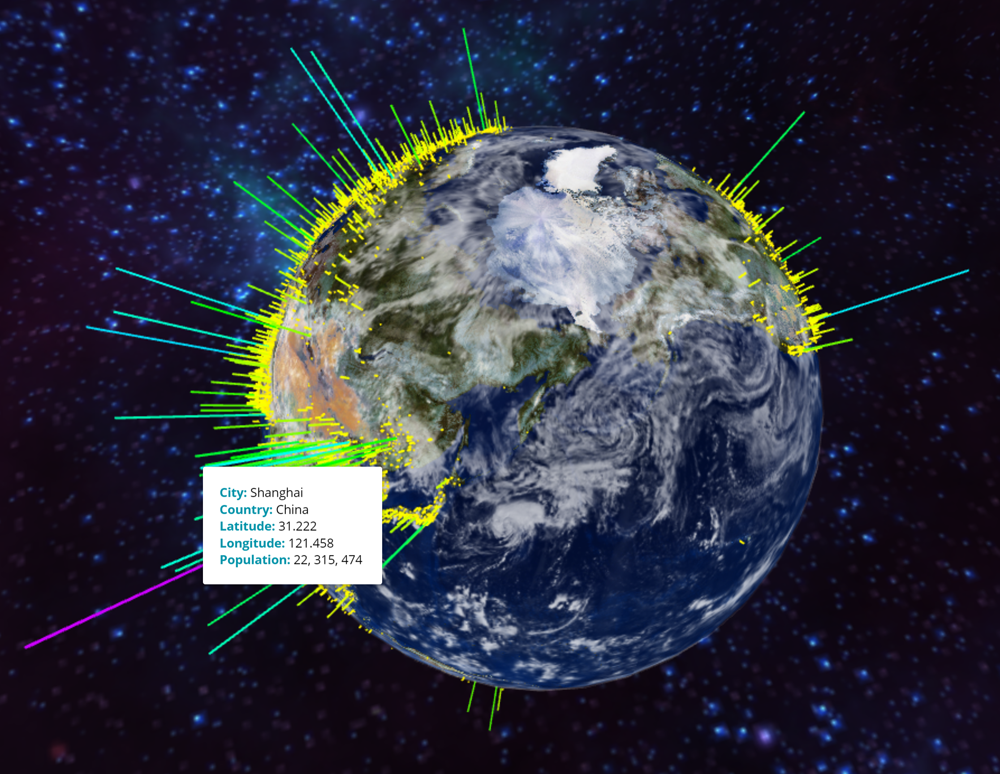
\includegraphics[width=\textwidth]{images/implementation/filtering/information_after}}
		\caption{After filtering information.}
		\label{fig:after_filtering_information}
	\end{subfigure}
	\caption[Filtering comparison]{Filtering comparison.}
	\label{fig:filtering_comparison}
\end{figure}
